\chapter{Theoretical framework}


\section{About LiF:Mg,Ti} \label{sec:LiF}


Lithium fluoride (LiF) is a crystalline material that has been widely used in radiation dosimetry due to its favorable % !!!!
properties. It first appeared as a thermoluminescent dosimetry material in the 1950's, and since then, it has been extensively studied in the field of radiation detection. The material is composed of lithium (Li) and fluor (F) %?????
atoms, forming a crystal lattice structure of a face-centered cubic (FCC) type. Without any impurities, LiF is a semiconductor, with a bandgap of approximately 14 eV, which makes it an excellent insulator at room temperature.

\vspace{10pt}

To enhance the properties for radiation detection, LiF is often doped with magnesium (Mg) and titanium (Ti) ions, and sold commercially as TLD-100 \cite{lif}. The doping process introduces defects in the crystal lattice, creating energy levels within the bandgap. These defects play a crucial role in trapping and releasing charge carriers, which are responsible for the thermoluminescent response of the material. This process is known as thermoluminescence (TL), where the trapped electrons are released upon heating, resulting in the emission of light. The intensity of this emitted light is proportional to the amount of radiation absorbed by the material, making it a valuable tool for dosimetry.




\section{The mathematical model} \label{sec:modelo}

To describe the thermoluminescent response of a semicoductor, we can use a mathematical model based on the trapping and releasing of charge carriers in the accesible energy levels of the material. 

\vspace{10pt}

Let us first consider the case of an arbitrary semicoductor without impurities. The energy levels of the conduction band and the valence band are separated by a bandgap $E_g$, and can be obtained with Schrodinger's equation that is under the influence of a periodic potential:

\begin{equation} \label{eq:schrodinger}
  \left[ -\frac{\hbar^2}{2m} \nabla^2 + V(\vec{r}) \right] \psi(\vec{r}) = E ~ \psi(\vec{r}),
\end{equation}

\vspace{10pt}
The periodicity of the potential $V(\vec{r})$ for any lattice vector $\vec{R}$ allows the Bloch's theorem to apply, and so it gives rise to the formation of a band structure, composed by the conduction band, which is typically fully occupied at absolute zero temperature, and the valence band, which is in turn typically empty -or rather, we can consider it filled with holes ($h^+$), or ``positively charged electrons''. The bandgap $E_g$ is then defined as the energy difference between the top of the valence band and the bottom of the conduction band, and for a perfect crystal, no energy states are allowed in that region. This can be clearly seen if we take into account the density of available states, $D(E)$, which is a function of the Fermi-Dirac distribution $f(E)$ for a certain temperature $T$. This function gives the occupancy of any energy level $E$, and can be expressed as:

\begin{equation} \label{eq:fermidirac}
  f(E) = \frac{1}{e^{\frac{E - E_f}{k_B T}} + 1},
\end{equation}

Where $E_f$ is the Fermi Level, and $k_B$ is the Boltzmann constant. If the system is in equilibrium, and we set the case of $T=0K$, the occupancy function $f(E)$ will be equal to 1 for all energy levels below the Fermi level, and 0 for all energy levels above it. This means that the occupancy function will be a step function, with a discontinuity at the Fermi level, and so we can see that there are no available states in the bandgap region.

\begin{figure}[H]
  \centering
  
\includegraphics[width=0.8\textwidth]{Images/FD_irradiation.png}
  \caption{Fermi-Dirac distribution for a semicoductor that is irradiated.}
  \label{fig:FD_irradiation}
\end{figure}


\vspace{10pt}
The introduction of impurities or defects however, break the periodicity of the lattice, and create localized energy levels inside this ``forbidden region''. These levels can be thought of as traps for electrons if we are situated above the fermi level, and traps of holes if we are situated below. When this material is irradiated, electrons from the valence band can be excited to the conduction band, creating an electron-hole pair; and so changing the shape of the occupancy function. Once excited, both electrons and holes get ``trapped'' in these localized energy levels, and the excitation of these pairs into equilibrium will result in the emission of energy. In Figure \ref{fig:FD_irradiation} we can see a broad description of the perturbation of the system from its equilibrium state due to the irradiation, and the return of the system to equilibrium during either thermal stimulation or optical stimulation. If said relaxation processes are radiative, TL and OSL result. 

\begin{figure}[H]
  \centering
  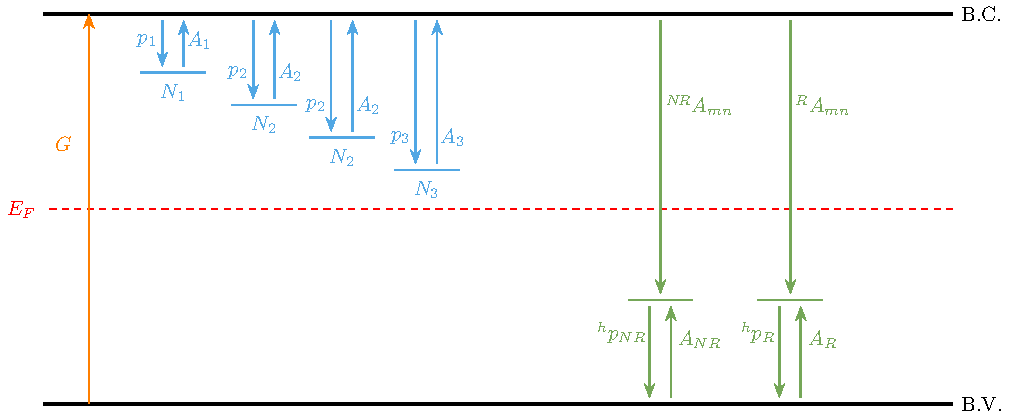
\includegraphics[width=0.8\textwidth]{Images/modeldiagram.pdf}
  \caption{Schematic representation of the theoretical model.}
  \label{fig:TheoreticalModel}
\end{figure}

And so, we can se a schematic representation of our theoretical model in Figure \ref{fig:TheoreticalModel}. Situating the energy in the Y axis, the focus is set in the energy gap of our material. Drawn in blue 






\vspace{10pt}








\section{The frequency factor} \label{sec:factorfrecuencia}

